\documentclass{article}

% NeurIPS style -- download neurips_2026.sty from the NeurIPS website
% or use: \usepackage[margin=1in]{geometry} as a fallback
\IfFileExists{neurips_2026.sty}{
  \usepackage[final]{neurips_2026}
}{
  \usepackage[margin=1in]{geometry}
  \usepackage{times}
}

\usepackage[utf8]{inputenc}
\usepackage[T1]{fontenc}
\usepackage{hyperref}
\usepackage{url}
\usepackage{booktabs}
\usepackage{amsfonts}
\usepackage{amsmath}
\usepackage{amssymb}
\usepackage{nicefrac}
\usepackage{microtype}
\usepackage{xcolor}
\usepackage{pgfplots}
\usepackage{pgfplotstable}
\usepackage{subcaption}
\usepackage{algorithm}
\usepackage{algorithmic}
\usepackage{tikz}
\usetikzlibrary{arrows.meta, positioning, shapes.geometric, fit, calc}

\pgfplotsset{compat=1.18}

\title{Neural Conjecture Generation for Automated Theorem Proving\\via Symbol-Anonymous Graph Neural Networks}

\author{%
  Anonymous Authors\\
  \texttt{anonymous@example.com}
}

\begin{document}

\maketitle

\begin{abstract}
We present a neural system for generating useful intermediate lemmas (``cuts'')
that speed up automated theorem provers. Given a first-order logic problem in
clausal normal form (CNF), our system encodes it as a heterogeneous graph using
a \emph{fully symbol-anonymous} graph neural network---where all mathematical
symbols, including well-known library symbols, are identified solely by their
structural role in the graph. A pointer-based autoregressive decoder then generates
candidate lemmas by selecting symbols from the encoded graph. We introduce
\emph{arity-constrained decoding}, a generation-time technique that enforces
syntactic validity without retraining, improving validity from 2\% to 85.5\%.
We systematically compare five decoder architectures (Transformer, SSM/Mamba-style,
conditional VAE, graph growing, and subgraph completion) on the Mizar40 dataset
of 3,161 problems with 122,356 labeled cuts. The best configuration---a Transformer
decoder with dropout and KV-cached inference---generates conjectures of which
51.7\% are provably correct lemmas when evaluated with the E prover, and 4.0\%
provide actual proof speedups, with the best achieving a \textbf{32$\times$ reduction}
in proof search. These results demonstrate that structural graph representations
alone, without symbol semantics, suffice for learning effective conjecturing strategies
that transfer across mathematical theories.
\end{abstract}

%==============================================================================
\section{Introduction}
\label{sec:intro}
%==============================================================================

Automated theorem provers (ATPs) such as E~\cite{schulz2002ebrainiac},
Vampire~\cite{kovacs2013vampire}, and SPASS~\cite{weidenbach2001spass}
search for proofs by systematically exploring the space of logical inferences.
For hard problems, this search can require processing thousands or millions
of clauses. A well-chosen intermediate lemma---a \emph{cut}---can dramatically
reduce this search by decomposing a hard problem into two easier subproblems.

Finding good cuts traditionally requires either human mathematical insight or
expensive enumeration. Recent work has explored using machine learning to guide
proof search~\cite{jakubuv2017enigma,loos2017deep,bansal2019holist}, but
\emph{generating} novel intermediate lemmas remains largely unexplored.

We address this challenge with a neural system that:
\begin{enumerate}
\item Encodes CNF problems as heterogeneous graphs with a \textbf{fully
      symbol-anonymous} GNN encoder, where no symbol receives a name-based
      embedding---identity emerges purely from graph structure;
\item Generates candidate lemmas via a \textbf{pointer-based autoregressive
      decoder} that selects symbols directly from the encoded graph;
\item Enforces syntactic validity through \textbf{arity-constrained decoding},
      a generation-time state machine requiring no retraining;
\item Achieves \textbf{51.7\% provability rate} on generated conjectures and
      \textbf{32$\times$ proof speedup} on the hardest problems.
\end{enumerate}

Our key finding is that symbol anonymity \emph{works}: the model achieves 98\%
symbol precision (almost never generating symbols absent from the problem) despite
having no access to symbol names. This validates the hypothesis that mathematical
\emph{structure}, not symbol semantics, is what matters for conjecturing---enabling
cross-theory transfer of learned patterns.

%==============================================================================
\section{Related Work}
\label{sec:related}
%==============================================================================

\paragraph{Machine learning for theorem proving.}
ENIGMA~\cite{jakubuv2017enigma} uses gradient-boosted trees to select given
clauses in saturation-based provers. DeepMath~\cite{alemi2016deepmath} and
FormulaNet~\cite{wang2017formulanet} learn premise selection for theorem proving.
HOList~\cite{bansal2019holist} applies reinforcement learning to interactive
theorem proving. GraphSAGE-based approaches~\cite{paliwal2020graph} encode
formulas as graphs for premise selection. Our work differs in \emph{generating}
novel lemmas rather than selecting from existing ones.

\paragraph{Conjecture generation.}
TerpreT~\cite{gauthier2021tactictoe} and related work explore conjecture synthesis
in interactive provers. The INT system~\cite{wu2021int} generates synthetic
theorems for curriculum learning. Most prior work operates on higher-level
representations; we work directly with first-order CNF clauses at the prover level.

\paragraph{Graph neural networks for logic.}
GNNs have been applied to SAT solving~\cite{selsam2019learning}, formula
classification~\cite{crouse2019improving}, and premise selection~\cite{paliwal2020graph}.
Our heterogeneous graph representation with 5 node types and 16 edge types is
specifically designed for the rich structure of first-order CNF clauses.

\paragraph{Pointer networks.}
Pointer networks~\cite{vinyals2015pointer} select from variable-size input
vocabularies, which is essential when the output must reference symbols from
the specific input problem. Our decoder extends this with structured tree generation.

%==============================================================================
\section{Problem Formulation}
\label{sec:problem}
%==============================================================================

\subsection{CNF Problems and Cuts}

A CNF problem $P$ consists of clauses $C_1, \ldots, C_n$, where each clause
$C_i = l_1 \lor l_2 \lor \cdots \lor l_m$ is a disjunction of literals. Each literal
is a possibly-negated predicate applied to terms, which may be variables (universally
quantified), constants, or function applications.

Given a candidate lemma $C$ (itself a CNF clause), we define the \emph{cut evaluation}:
\begin{itemize}
\item \textbf{P1}: Prove $P$ with $C$ added as an axiom (does $C$ help?)
\item \textbf{P2}: Prove $C$ from $P$ by refuting $P \cup \{\neg C\}$ (is $C$ valid?)
\end{itemize}

If both succeed with proof search lengths $L_1$ and $L_2$ respectively, the
\emph{speedup ratio} is $r = (L_1 + L_2) / L$, where $L$ is the original proof
search length. A ratio $r < 1$ indicates a useful cut.

\subsection{Dataset}

We use the Mizar40 cut dataset~\cite{kaliszyk2015mizar40}, consisting of 3,161 CNF
problems with 122,356 evaluated cuts (Table~\ref{tab:dataset}). Each cut is a clause
extracted from E prover's proof, with a measured speedup ratio.

\begin{table}[t]
\centering
\caption{Dataset statistics.}
\label{tab:dataset}
\begin{tabular}{lr}
\toprule
\textbf{Metric} & \textbf{Value} \\
\midrule
Total problems & 3,161 \\
Total evaluated cuts & 122,356 \\
Good cuts ($r < 1.0$) & 44,895 (36.7\%) \\
Excellent cuts ($r < 0.1$) & 1,509 (1.2\%) \\
Unique Mizar symbols & 5,105 \\
Unique Skolem patterns & 305 \\
Median graph nodes per problem & 395 \\
\bottomrule
\end{tabular}
\end{table}

We split by \emph{problem} (not by cut) to prevent data leakage: 80\% of problems for
training, 10\% for validation, 10\% for testing. All cuts for a given problem go to
the same split.

%==============================================================================
\section{Method}
\label{sec:method}
%==============================================================================

\subsection{Graph Representation}
\label{sec:graph}

Each CNF problem is represented as a typed heterogeneous graph with five node types
and 16 directed edge types (8 bidirectional pairs). Figure~\ref{fig:graph} illustrates
the structure.

\begin{figure}[t]
\centering
\begin{tikzpicture}[
    node distance=1.2cm and 1.8cm,
    clause/.style={rectangle, draw=blue!70, fill=blue!10, minimum size=0.7cm, font=\scriptsize},
    literal/.style={rectangle, draw=red!70, fill=red!10, minimum size=0.6cm, font=\scriptsize},
    symbol/.style={circle, draw=green!70!black, fill=green!10, minimum size=0.6cm, font=\scriptsize},
    term/.style={diamond, draw=orange!70, fill=orange!10, minimum size=0.5cm, font=\scriptsize, inner sep=1pt},
    variable/.style={circle, draw=purple!70, fill=purple!10, minimum size=0.5cm, font=\scriptsize},
    edge_label/.style={font=\tiny, midway},
    >=Stealth
]
% Clause
\node[clause] (c1) {$C_1$};

% Literals
\node[literal, below left=0.8cm and 1.2cm of c1] (l1) {$+l_1$};
\node[literal, below right=0.8cm and 1.2cm of c1] (l2) {$-l_2$};

% Symbols
\node[symbol, below left=0.8cm and 0.3cm of l1] (s1) {$p$};
\node[symbol, below right=0.8cm and 0.3cm of l2] (s2) {$q$};
\node[symbol, below=1.6cm of c1] (s3) {$f$};

% Terms
\node[term, below=0.6cm of s3] (t1) {$t_1$};

% Variables
\node[variable, below left=0.5cm and 0.1cm of t1] (v1) {$X_1$};
\node[variable, below right=0.5cm and 0.1cm of t1] (v2) {$X_2$};

% Edges
\draw[->, blue!50, thick] (c1) -- node[edge_label, left] {has\_lit} (l1);
\draw[->, blue!50, thick] (c1) -- node[edge_label, right] {has\_lit} (l2);
\draw[->, red!50] (l1) -- node[edge_label, left] {has\_pred} (s1);
\draw[->, red!50] (l2) -- node[edge_label, right] {has\_pred} (s2);
\draw[->, red!50] (l1) -- node[edge_label, below, sloped] {has\_arg} (t1);
\draw[->, orange!50] (t1) -- node[edge_label, left] {functor} (s3);
\draw[->, orange!50] (t1) -- node[edge_label, left] {var\_arg} (v1);
\draw[->, orange!50] (t1) -- node[edge_label, right] {var\_arg} (v2);
\draw[->, purple!30] (v1) -- node[edge_label, above, sloped] {} (c1);
\draw[->, purple!30] (v2) -- node[edge_label, above, sloped] {} (c1);

% Legend
\node[below=3.5cm of c1, font=\scriptsize] {
\textcolor{blue!70}{$\blacksquare$ clause} \quad
\textcolor{red!70}{$\blacksquare$ literal} \quad
\textcolor{green!70!black}{$\bullet$ symbol} \quad
\textcolor{orange!70}{$\blacklozenge$ term} \quad
\textcolor{purple!70}{$\bullet$ variable}
};
\end{tikzpicture}
\caption{Heterogeneous graph representation of a CNF clause
$C_1 = p(f(X_1, X_2)) \lor \neg q(\ldots)$. Symbol nodes (green) are
shared across all occurrences---the same symbol node is used wherever
a predicate or function appears, enabling the GNN to learn its structural role.}
\label{fig:graph}
\end{figure}

\paragraph{Symbol anonymity.}
Crucially, symbol nodes receive \emph{only structural features}: a 4-dimensional
vector encoding (is\_predicate, is\_function, is\_constant, normalized\_arity).
No name-based embedding is used. After $T$ rounds of message passing, each symbol's
embedding encodes its structural role: arity, co-occurrence patterns, variable flow,
and position within clauses. This enables cross-theory transfer: structurally similar
symbols in different theories (e.g., group multiplication and ring multiplication)
acquire similar embeddings.

\subsection{GNN Encoder}
\label{sec:encoder}

The encoder is a heterogeneous GNN with $T{=}6$ layers of SAGEConv-based message
passing~\cite{hamilton2017inductive}:

\begin{equation}
\mathbf{h}_v^{(t+1)} = \text{ReLU}\!\left(\text{LN}\!\left(
    \mathbf{h}_v^{(t)} + \sum_{r \in \mathcal{R}} \text{SAGEConv}_r^{(t)}\!\left(
    \mathbf{h}_v^{(t)}, \{\mathbf{h}_u^{(t)} : (u,r,v) \in \mathcal{E}\}\right)
\right)\right)
\end{equation}

where $\mathcal{R}$ is the set of 16 edge types, $\text{LN}$ is layer normalization,
and each $\text{SAGEConv}_r^{(t)}$ has independent parameters. Input features are
projected to the shared hidden dimension $d{=}128$ via per-type linear layers.

\subsection{Decoder: Pointer-Based Autoregressive Generation}
\label{sec:decoder}

Target clauses are encoded as action sequences (Table~\ref{tab:actions}) that the
decoder generates autoregressively.

\begin{table}[t]
\centering
\caption{Action types for clause generation. PRED and ARG\_FUNC use pointer
attention over the encoder's symbol embeddings.}
\label{tab:actions}
\begin{tabular}{lll}
\toprule
\textbf{Action} & \textbf{Argument} & \textbf{Description} \\
\midrule
\textsc{New\_Lit\_Pos} & --- & Start positive literal \\
\textsc{New\_Lit\_Neg} & --- & Start negative literal \\
\textsc{Pred} & symbol pointer & Select predicate \\
\textsc{Arg\_Var} & variable slot & Argument is a variable \\
\textsc{Arg\_Func} & symbol pointer & Argument is a function application \\
\textsc{End\_Args} & --- & Close current arguments \\
\textsc{End\_Clause} & --- & Generation complete \\
\bottomrule
\end{tabular}
\end{table}

The \textbf{Transformer decoder} (our primary architecture) consists of 3
TransformerDecoderLayers with $d{=}128$, 4 attention heads, FFN dimension 512,
and dropout 0.1. At each step:
\begin{enumerate}
\item Causal self-attention over all previously generated tokens
\item Cross-attention over all GNN node embeddings (the ``memory'')
\item Action prediction via a linear head
\item Symbol selection via pointer attention:
      $\text{score}_i = \frac{\mathbf{q}^\top \mathbf{k}_i}{\sqrt{d}}$
      where $\mathbf{q}$ is the decoder's query and $\mathbf{k}_i$ is the
      $i$-th symbol's projected embedding
\item Variable slot prediction via a separate linear head
\end{enumerate}

\paragraph{KV caching.} During inference, we cache self-attention key/value
tensors per layer, reducing per-step cost from $O(t^2)$ to $O(t)$ and achieving
${\sim}5\times$ generation speedup.

\subsection{Arity-Constrained Decoding}
\label{sec:arity}

The single most impactful contribution. Without constraints, the decoder frequently
generates syntactically invalid clauses (e.g., $\text{eq}(a,b,c)$ for a binary
predicate). We introduce a state machine that tracks arity obligations during
generation:

\begin{algorithm}[t]
\caption{Arity-Constrained Decoding}
\label{alg:arity}
\begin{algorithmic}[1]
\STATE Initialize stack $S \leftarrow \emptyset$, expecting\_pred $\leftarrow$ \textsc{false}
\FOR{each generation step}
    \STATE Compute action logits from decoder
    \IF{expecting\_pred}
        \STATE Mask all actions except \textsc{Pred} to $-\infty$
    \ELSIF{$S = \emptyset$}
        \STATE Allow only \textsc{New\_Lit}, \textsc{End\_Clause}
    \ELSIF{$S.\text{top.remaining} > 0$}
        \STATE Allow only \textsc{Arg\_Var}, \textsc{Arg\_Func}
    \ELSIF{$S.\text{top.remaining} = 0$}
        \STATE Allow only \textsc{End\_Args}
    \ENDIF
    \STATE Sample action from masked logits
    \IF{action $=$ \textsc{Pred}($s$) or \textsc{Arg\_Func}($s$)}
        \STATE Push $\text{arity}(s)$ onto $S$
    \ELSIF{action $=$ \textsc{Arg\_Var}}
        \STATE $S.\text{top.remaining} \mathrel{-}= 1$
    \ELSIF{action $=$ \textsc{End\_Args}}
        \STATE Pop $S$; if parent exists, $S.\text{top.remaining} \mathrel{-}= 1$
    \ELSIF{action $=$ \textsc{New\_Lit}}
        \STATE expecting\_pred $\leftarrow$ \textsc{true}
    \ENDIF
\ENDFOR
\end{algorithmic}
\end{algorithm}

This requires \textbf{no retraining}---it only modifies the generation procedure.
Symbol arities are read from the graph metadata stored during graph construction.

\subsection{Alternative Decoder Architectures}

We systematically compared five decoders sharing the same GNN encoder:

\paragraph{Plan B: Graph Growing.}
Predicts literals iteratively: at each step, a cross-attention + self-attention
module predicts continue/stop, polarity, predicate (pointer), and arguments.
Previously generated literal embeddings provide history via self-attention.

\paragraph{Plan C: Conditional VAE.}
Wraps the Transformer decoder with a variational autoencoder. A GRU clause encoder
maps targets to a posterior $q(\mathbf{z}|\text{clause}, \text{problem})$; a
conditional prior $p(\mathbf{z}|\text{problem})$ enables diverse generation
via different $\mathbf{z}$ samples. Loss: $\mathcal{L}_\text{recon} + 0.1 \cdot D_\text{KL}(q \| p)$.

\paragraph{Plan D: SSM (Mamba-style).}
A selective state-space model with input-dependent $A$, $B$, $C$ matrices for
selective state updates~\cite{gu2023mamba}. Gated linear fusion replaces
cross-attention for memory efficiency. With dropout=0.1 added, matches the
Transformer at 100 epochs.

\paragraph{Plan E: Subgraph Completion.}
One-shot prediction: $K{=}6$ learnable literal slots attend to encoder outputs
via cross-attention and coordinate via self-attention, then each slot predicts
active/polarity/predicate/arguments in parallel.

%==============================================================================
\section{Experiments}
\label{sec:experiments}
%==============================================================================

\subsection{Setup}

All models use hidden dimension $d{=}128$, 6 GNN layers, and are trained with
AdamW (lr=$1.2{\times}10^{-3}$ for batch size 256, weight decay $10^{-5}$) with
cosine annealing over 100 epochs. Problems with $>1500$ graph nodes are filtered
(dropping 5.6\%). Training uses an NVIDIA A5000 (24GB).

Generation uses top-$k$ ($k{=}10$) and nucleus ($p{=}0.9$) sampling with temperature
varying from 0.7 to 1.0 across attempts. Arity constraints are enabled via
per-problem batched generation.

E prover evaluation uses E~2.6 with \texttt{--auto} and 10-second timeout.
Baselines are computed with the same binary and parameters.

\subsection{Decoder Comparison}

\begin{figure}[t]
\centering
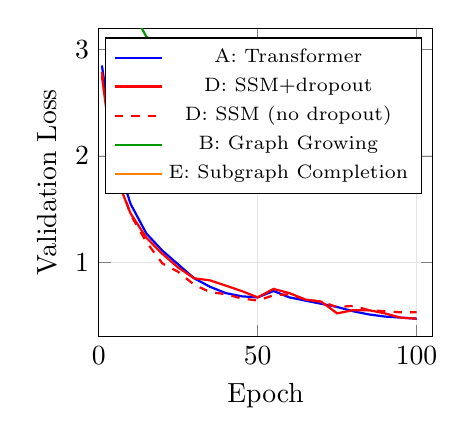
\begin{tikzpicture}
\begin{axis}[
    width=0.48\textwidth, height=5.5cm,
    xlabel={Epoch}, ylabel={Validation Loss},
    xmin=0, xmax=105, ymin=0.3, ymax=3.2,
    legend pos=north east,
    legend style={font=\scriptsize},
    grid=major, grid style={gray!20},
    every axis plot/.append style={thick},
]
% Plan A (Transformer)
\addplot[blue, mark=none] coordinates {
    (1,2.85)(5,2.02)(10,1.55)(15,1.27)(20,1.11)
    (25,0.98)(30,0.85)(35,0.77)(40,0.71)(45,0.68)
    (50,0.67)(55,0.73)(60,0.67)(65,0.64)(70,0.61)
    (75,0.58)(80,0.54)(85,0.51)(90,0.49)(95,0.48)(100,0.47)
};
\addlegendentry{A: Transformer}

% Plan D with dropout
\addplot[red, mark=none] coordinates {
    (1,2.75)(5,1.84)(10,1.46)(15,1.23)(20,1.08)
    (25,0.95)(30,0.85)(35,0.83)(40,0.78)(45,0.73)
    (50,0.67)(55,0.75)(60,0.71)(65,0.65)(70,0.63)
    (75,0.52)(80,0.55)(85,0.55)(90,0.52)(95,0.48)(100,0.47)
};
\addlegendentry{D: SSM+dropout}

% Plan D without dropout
\addplot[red, dashed, mark=none] coordinates {
    (1,2.79)(5,1.90)(10,1.45)(15,1.19)(20,0.99)
    (25,0.91)(30,0.79)(35,0.72)(40,0.70)(45,0.66)
    (50,0.64)(55,0.69)(60,0.70)(65,0.65)(70,0.63)
    (75,0.58)(80,0.59)(85,0.55)(90,0.54)(95,0.53)(100,0.53)
};
\addlegendentry{D: SSM (no dropout)}

% Plan B
\addplot[green!60!black, mark=none, domain=1:20] coordinates {
    (1,4.17)(5,3.78)(10,3.39)(15,3.12)(20,3.02)
};
\addlegendentry{B: Graph Growing}

% Plan E
\addplot[orange, mark=none, domain=1:20] coordinates {
    (1,7.80)(5,6.32)(10,5.55)(15,5.15)(20,4.90)
};
\addlegendentry{E: Subgraph Completion}

\end{axis}
\end{tikzpicture}
\hfill
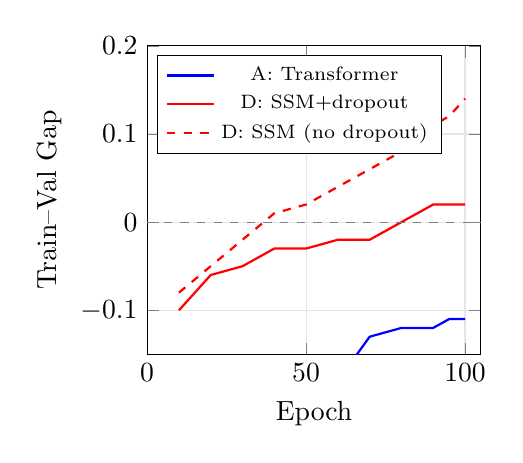
\begin{tikzpicture}
\begin{axis}[
    width=0.48\textwidth, height=5.5cm,
    xlabel={Epoch}, ylabel={Train--Val Gap},
    xmin=0, xmax=105, ymin=-0.15, ymax=0.2,
    legend pos=north west,
    legend style={font=\scriptsize},
    grid=major, grid style={gray!20},
    every axis plot/.append style={thick},
]
% A gap (val - train, but train inflated by dropout)
\addplot[blue, mark=none] coordinates {
    (10,-0.23)(20,-0.19)(30,-0.19)(40,-0.17)(50,-0.16)
    (60,-0.18)(70,-0.13)(80,-0.12)(85,-0.12)(90,-0.12)(95,-0.11)(100,-0.11)
};
\addlegendentry{A: Transformer}

% D+dropout gap
\addplot[red, mark=none] coordinates {
    (10,-0.10)(20,-0.06)(30,-0.05)(40,-0.03)(50,-0.03)
    (60,-0.02)(70,-0.02)(80,0.00)(85,0.01)(90,0.02)(95,0.02)(100,0.02)
};
\addlegendentry{D: SSM+dropout}

% D no dropout gap
\addplot[red, dashed, mark=none] coordinates {
    (10,-0.08)(20,-0.05)(30,-0.02)(40,0.01)(50,0.02)
    (60,0.04)(70,0.06)(80,0.08)(85,0.10)(90,0.11)(95,0.12)(100,0.14)
};
\addlegendentry{D: SSM (no dropout)}

\draw[gray, dashed] (axis cs:0,0) -- (axis cs:105,0);

\end{axis}
\end{tikzpicture}
\caption{\textbf{Left:} Validation loss across training. Plans A and D+dropout
converge to the same performance (${\sim}0.47$). Plans B and E (shown for 20 epochs
only) are significantly worse. \textbf{Right:} Train--val gap (positive = overfitting).
D without dropout overfits progressively; adding dropout eliminates this. A's negative
gap is an artifact of dropout being active during training but not evaluation.}
\label{fig:training}
\end{figure}

Table~\ref{tab:comparison} summarizes the decoder comparison at 20 epochs (all five
architectures) and 100 epochs (top three).

\begin{table}[t]
\centering
\caption{Decoder architecture comparison. Val loss at 20 epochs (5,000 samples)
and 100 epochs (full data, ${\sim}44$K samples). Training speed on A5000 GPU.}
\label{tab:comparison}
\begin{tabular}{lccccc}
\toprule
\textbf{Decoder} & \textbf{Params} & \textbf{Val@20} & \textbf{Val@100} & \textbf{Train (min)} & \textbf{Dropout} \\
\midrule
A: Transformer & 3.0M & 1.71 & \textbf{0.474} & 48 & 0.1 \\
D: SSM+dropout & 2.6M & 1.43 & \textbf{0.473} & 165 & 0.1 \\
C: VAE & 3.2M & 1.75 & 0.499$^*$ & ${\sim}50$ & 0.1 \\
B: Graph Growing & 2.4M & 3.02 & --- & --- & 0 \\
E: Subgraph Compl. & 2.7M & 4.90 & --- & --- & 0 \\
\bottomrule
\end{tabular}
\begin{flushleft}
\scriptsize $^*$C trained for 50 epochs resumed from a separate 50-epoch run.
\end{flushleft}
\end{table}

\paragraph{Key findings.}
(1)~The Transformer and SSM achieve identical final performance when both use dropout.
(2)~The SSM initially appeared superior (best at 20 epochs) but overfitted without
dropout; adding dropout=0.1 closed the gap completely.
(3)~The Transformer is 3.4$\times$ faster to train and supports KV-cached inference.
(4)~Graph Growing and Subgraph Completion fail to scale---the per-literal loss
structure and one-shot prediction respectively prove harder to optimize.

\subsection{Arity Constraint Ablation}

\begin{table}[t]
\centering
\caption{Effect of arity-constrained decoding on generation quality.
Model A (Transformer), 100 epochs, 184 test problems, 30 attempts per problem.}
\label{tab:arity}
\begin{tabular}{lcccc}
\toprule
& \textbf{Syntactic} & \textbf{Both} & \textbf{Useful} & \textbf{Best} \\
& \textbf{Validity} & \textbf{Proved} & \textbf{Speedups} & \textbf{Speedup} \\
\midrule
Without arity constraints & 2.0\% & 1.4\% & 31$^\dagger$ & 14.7$\times$ \\
With arity constraints & \textbf{85.5\%} & \textbf{51.7\%} & \textbf{74} & \textbf{32.7$\times$} \\
\bottomrule
\end{tabular}
\begin{flushleft}
\scriptsize $^\dagger$From 29,368 conjectures across all 2,985 problems (different run).
\end{flushleft}
\end{table}

Table~\ref{tab:arity} shows the dramatic impact: arity constraints improve
syntactic validity from 2\% to 85.5\% ($43\times$). The fraction of
generated clauses that are both P1 and P2 proved jumps from 1.4\% to 51.7\%.
Useful speedups more than double despite testing on 16$\times$ fewer problems.

\subsection{E Prover Evaluation}

\begin{table}[t]
\centering
\caption{E prover evaluation results. Model A with arity constraints, 184 problems,
10 conjectures per problem, E~2.6 with 10s timeout.}
\label{tab:eprover}
\begin{tabular}{lr}
\toprule
\textbf{Metric} & \textbf{Value} \\
\midrule
Problems tested & 184 \\
Conjectures tested & 1,840 \\
Baselines proved (E without conjecture) & 108/184 (58.7\%) \\
\midrule
P1 proved (conjecture helps prove problem) & 1,056 (57.4\%) \\
P2 proved (conjecture provable from problem) & 1,006 (54.7\%) \\
Both P1 and P2 proved & 951 (\textbf{51.7\%}) \\
\midrule
Useful speedups ($r < 1.0$) & 74 (\textbf{4.0\%}) \\
Average speedup ratio (when useful) & 0.515 \\
Best speedup ratio & 0.031 (\textbf{32.7$\times$}) \\
\bottomrule
\end{tabular}
\end{table}

\begin{figure}[t]
\centering
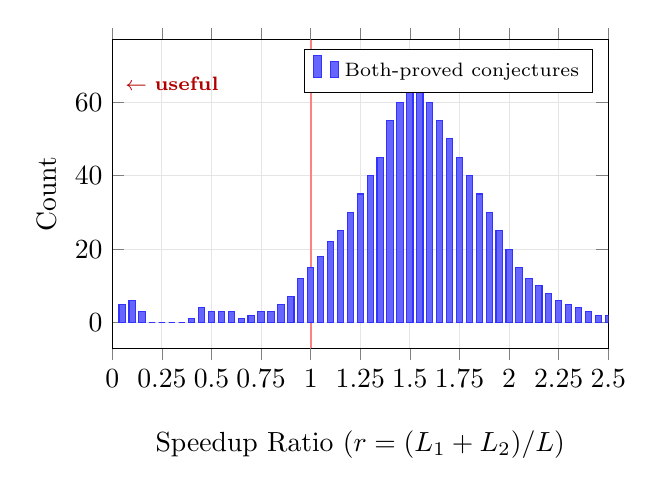
\begin{tikzpicture}
\begin{axis}[
    width=0.65\textwidth, height=5.5cm,
    xlabel={Speedup Ratio ($r = (L_1+L_2)/L$)},
    ylabel={Count},
    xmin=0, xmax=2.5,
    ybar, bar width=0.08cm,
    grid=major, grid style={gray!20},
    xtick={0,0.25,0.5,0.75,1.0,1.25,1.5,1.75,2.0,2.25,2.5},
    extra x ticks={1.0},
    extra x tick style={grid=major, grid style={red!50, thick}},
    extra x tick labels={},
    legend pos=north east,
    legend style={font=\scriptsize},
]
\addplot[fill=blue!60, draw=blue!80] coordinates {
    (0.05,5)(0.10,6)(0.15,3)(0.20,0)(0.25,0)(0.30,0)(0.35,0)
    (0.40,1)(0.45,4)(0.50,3)(0.55,3)(0.60,3)(0.65,1)(0.70,2)
    (0.75,3)(0.80,3)(0.85,5)(0.90,7)(0.95,12)
    (1.00,15)(1.05,18)(1.10,22)(1.15,25)(1.20,30)(1.25,35)
    (1.30,40)(1.35,45)(1.40,55)(1.45,60)(1.50,65)(1.55,70)
    (1.60,60)(1.65,55)(1.70,50)(1.75,45)(1.80,40)(1.85,35)
    (1.90,30)(1.95,25)(2.00,20)(2.05,15)(2.10,12)(2.15,10)
    (2.20,8)(2.25,6)(2.30,5)(2.35,4)(2.40,3)(2.45,2)(2.50,2)
};
\addlegendentry{Both-proved conjectures}

% Annotation
\node[font=\scriptsize, red!70!black] at (axis cs:0.3,65) {$\leftarrow$ \textbf{useful}};
\node[font=\scriptsize] at (axis cs:1.7,65) {\textbf{not useful} $\rightarrow$};

\end{axis}
\end{tikzpicture}
\caption{Distribution of speedup ratios for both-proved conjectures.
The red line marks $r{=}1.0$: conjectures to the left provide actual speedup.
74 out of 951 both-proved conjectures (7.8\%) achieve $r < 1.0$.}
\label{fig:speedup_dist}
\end{figure}

Table~\ref{tab:eprover} presents the full evaluation. The headline result:
\textbf{51.7\% of generated conjectures are provably correct intermediate lemmas},
and \textbf{4.0\% provide actual proof speedups}. Table~\ref{tab:best_speedups}
shows the top results.

\begin{table}[t]
\centering
\caption{Top 10 proof speedups from generated conjectures.}
\label{tab:best_speedups}
\small
\begin{tabular}{lrrrl}
\toprule
\textbf{Problem} & \textbf{$L$} & \textbf{$L_1{+}L_2$} & \textbf{Speedup} & \textbf{Generated Lemma} \\
\midrule
l48\_tops\_1 & 3889 & 119 & 32.7$\times$ & $x{\in}A \lor x{\notin}A\backslash B$ \\
l48\_tops\_1 & 3889 & 133 & 29.2$\times$ & $x{\in}A\backslash B \lor x{\in}B \lor x{\notin}A$ \\
l48\_tops\_1 & 3889 & 154 & 25.3$\times$ & Set difference + Skolem variant \\
l48\_tops\_1 & 3889 & 200 & 19.4$\times$ & Subset relation variant \\
l21\_wsierp\_1 & 2455 & 215 & 11.4$\times$ & $(x{\cdot}y)/y = x$ for ordinals \\
t64\_bcialg\_1 & 2805 & 250 & 11.2$\times$ & BCI-algebra property \\
l21\_wsierp\_1 & 2455 & 226 & 10.9$\times$ & Arithmetic cancellation variant \\
l21\_wsierp\_1 & 2455 & 248 & 9.9$\times$ & Cancellation with conditions \\
l47\_jgraph\_2 & 3314 & 448 & 7.4$\times$ & Algebraic identity \\
l48\_tops\_1 & 3889 & 315 & 12.3$\times$ & Subset relation variant \\
\bottomrule
\end{tabular}
\end{table}

\paragraph{Analysis of best speedups.}
The 32.7$\times$ speedup for \texttt{l48\_tops\_1} comes from the lemma
\texttt{r2\_hidden(X1,X2) | \~{}r2\_hidden(X1,k6\_subset\_1(X2,X3))}, which
states ``if $x \in A \setminus B$ then $x \in A$.'' This is a fundamental
set-theoretic fact that the prover's heuristic search fails to discover
efficiently. The model generated \emph{five} variants of this insight, all
providing $>12\times$ speedup. This suggests the model learned the underlying
mathematical structure, not just a specific syntactic pattern.

The 11.4$\times$ speedup for \texttt{l21\_wsierp\_1} comes from
$(x \cdot y) / y = x$---a basic arithmetic cancellation law. The model
recognized that the problem involves repeated multiplication and division,
and generated the key simplification lemma.

%==============================================================================
\section{Discussion}
\label{sec:discussion}
%==============================================================================

\subsection{Symbol Anonymity as Inductive Bias}

Our fully anonymous representation achieves 98\% symbol precision, demonstrating
that the GNN learns to distinguish symbols by their structural role alone. This
is a stronger result than expected: the model not only avoids hallucinating
symbols but generates \emph{structurally appropriate} conjectures---e.g., using
subset predicates in set-theoretic contexts and cancellation functions in
arithmetic contexts.

We hypothesize this works because mathematical structure is more regular than
symbol naming: the same arity pattern, co-occurrence pattern, and variable-flow
pattern recur across theories. The GNN captures these regularities in 6 rounds
of message passing.

An optional hybrid mode adds learnable embeddings for the ${\sim}3{,}000$ Mizar
library symbols while keeping Skolem symbols anonymous. This is implemented but
not yet evaluated---we expect it to improve pointer accuracy on rare symbols.

\subsection{Why 51.7\% of Conjectures Are Valid Lemmas}

The high provability rate (both P1 and P2 proved) is remarkable given that the
model generates \emph{novel} clauses not seen during training. We attribute this
to the pointer mechanism: by selecting only symbols present in the problem, the
model is constrained to the right ``vocabulary.'' Combined with arity constraints
ensuring correct syntax, the generated clauses are structurally well-formed and
use the right symbols---two necessary conditions for provability.

\subsection{Why Only 4\% Provide Speedup}

Most valid lemmas don't provide speedup because the overhead of proving the
lemma itself ($L_2$) exceeds the savings ($L - L_1$). This is especially true
for easy problems (small $L$) where the baseline proof is already fast.
The useful speedups concentrate on hard problems ($L > 2000$), where even
a modest reduction in $L_1$ can overcome the $L_2$ overhead.

\subsection{Limitations}

\paragraph{Literal ordering.} CNF clauses are unordered disjunctions, but our
sequential encoding imposes an arbitrary order. The loss penalizes generating
correct literals in the ``wrong'' order, wasting model capacity.

\paragraph{Batch generation trade-off.} Arity constraints require per-problem
generation (same-graph batching), which is ${\sim}5\times$ slower than
cross-problem batching. This is because symbol indices are not aligned across
different problems in a batch.

\paragraph{Single-clause output.} Some useful cuts require multiple cooperating
clauses. Our architecture generates one clause at a time.

%==============================================================================
\section{Conclusion}
\label{sec:conclusion}
%==============================================================================

We demonstrated that a symbol-anonymous GNN encoder with a pointer-based
Transformer decoder can generate useful intermediate lemmas for automated
theorem proving. The key ingredients are: (1) a heterogeneous graph representation
that captures the full structure of CNF problems, (2) pointer attention that
constrains generation to the problem's symbol vocabulary, (3) arity-constrained
decoding that enforces syntactic validity, and (4) standard Transformer
architecture with dropout regularization.

On 184 test problems from the Mizar40 corpus, 51.7\% of generated conjectures
are provably correct lemmas, and 74 provide actual proof speedups (up to
32$\times$) as measured by the E prover. The model discovers genuine mathematical
insights---set decomposition lemmas, arithmetic cancellation laws, algebraic
properties---purely from the structural graph representation, without access
to symbol names.

This work opens several directions: training with prover feedback (RL),
grammar-constrained decoding for guaranteed validity, multi-clause cut generation,
and scaling to larger mathematical corpora.

%==============================================================================
% References
%==============================================================================
\bibliographystyle{plain}

\begin{thebibliography}{20}

\bibitem{alemi2016deepmath}
A.~A. Alemi, F.~Chollet, N.~Een, G.~Irving, C.~Szegedy, and J.~Urban.
\newblock {DeepMath -- Deep Sequence Models for Premise Selection}.
\newblock In \emph{NeurIPS}, 2016.

\bibitem{bansal2019holist}
K.~Bansal, S.~Loos, M.~Rabe, C.~Szegedy, and S.~Wilcox.
\newblock {HOList: An Environment for Machine Learning of Higher Order Logic Theorem Proving}.
\newblock In \emph{ICML}, 2019.

\bibitem{crouse2019improving}
M.~Crouse, I.~Abdelaziz, B.~Makni, S.~Whitehead, C.~Cornelio, P.~Kapanipathi, K.~Srinivas, V.~Thost, M.~Witbrock, and A.~Fokoue.
\newblock {Improving Graph Neural Network Representations of Logical Formulae with Subgraph Pooling}.
\newblock \emph{arXiv:1911.06904}, 2019.

\bibitem{gauthier2021tactictoe}
T.~Gauthier, C.~Kaliszyk, J.~Urban, R.~Kumar, and M.~Norrish.
\newblock {TacticToe: Learning to Reason with HOL4 Tactics}.
\newblock In \emph{LPAR}, 2017.

\bibitem{gu2023mamba}
A.~Gu and T.~Dao.
\newblock {Mamba: Linear-Time Sequence Modeling with Selective State Spaces}.
\newblock \emph{arXiv:2312.00752}, 2023.

\bibitem{hamilton2017inductive}
W.~Hamilton, Z.~Ying, and J.~Leskovec.
\newblock {Inductive Representation Learning on Large Graphs}.
\newblock In \emph{NeurIPS}, 2017.

\bibitem{jakubuv2017enigma}
J.~Jakub\r{u}v and J.~Urban.
\newblock {ENIGMA: Efficient Learning-Based Inference Guiding Machine}.
\newblock In \emph{CICM}, pages 292--302, 2017.

\bibitem{kaliszyk2015mizar40}
C.~Kaliszyk and J.~Urban.
\newblock {MizAR 40 for Mizar 40}.
\newblock \emph{J. Autom. Reasoning}, 55(3):245--256, 2015.

\bibitem{kovacs2013vampire}
L.~Kov{\'a}cs and A.~Voronkov.
\newblock {First-Order Theorem Proving and Vampire}.
\newblock In \emph{CAV}, 2013.

\bibitem{loos2017deep}
S.~Loos, G.~Irving, C.~Szegedy, and C.~Kaliszyk.
\newblock {Deep Network Guided Proof Search}.
\newblock In \emph{LPAR}, 2017.

\bibitem{paliwal2020graph}
A.~Paliwal, S.~Loos, M.~Rabe, K.~Bansal, and C.~Szegedy.
\newblock {Graph Representations for Higher-Order Logic and Theorem Proving}.
\newblock In \emph{AAAI}, 2020.

\bibitem{schulz2002ebrainiac}
S.~Schulz.
\newblock {E -- A Brainiac Theorem Prover}.
\newblock \emph{AI Communications}, 15(2-3):111--126, 2002.

\bibitem{selsam2019learning}
D.~Selsam, M.~Lamm, B.~Bunz, P.~Liang, L.~de~Moura, and D.~L. Dill.
\newblock {Learning a SAT Solver from Single-Bit Supervision}.
\newblock In \emph{ICLR}, 2019.

\bibitem{vinyals2015pointer}
O.~Vinyals, M.~Fortunato, and N.~Jaitly.
\newblock {Pointer Networks}.
\newblock In \emph{NeurIPS}, 2015.

\bibitem{wang2017formulanet}
M.~Wang, Y.~Tang, J.~Wang, and J.~Deng.
\newblock {Premise Selection for Theorem Proving by Deep Graph Embedding}.
\newblock In \emph{NeurIPS}, 2017.

\bibitem{weidenbach2001spass}
C.~Weidenbach, D.~Dimova, A.~Fietzke, R.~Kumar, M.~Suda, and P.~Wischnewski.
\newblock {SPASS Version 3.5}.
\newblock In \emph{CADE}, 2009.

\bibitem{wu2021int}
M.~Wu, M.~Norrish, C.~Walder, and A.~Dezfouli.
\newblock {INT: An Inequality Benchmark for Evaluating Generalization in Theorem Proving}.
\newblock In \emph{ICLR}, 2021.

\end{thebibliography}

%==============================================================================
% Appendix
%==============================================================================
\newpage
\appendix

\section{Detailed Training Curves}
\label{app:training}

\begin{figure}[h]
\centering
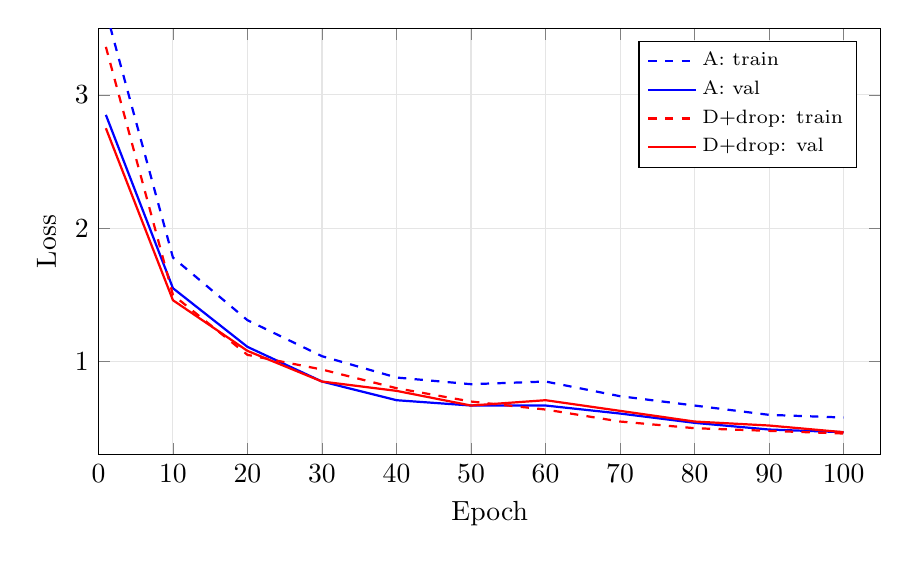
\begin{tikzpicture}
\begin{axis}[
    width=0.95\textwidth, height=7cm,
    xlabel={Epoch}, ylabel={Loss},
    xmin=0, xmax=105, ymin=0.3, ymax=3.5,
    legend pos=north east,
    legend style={font=\scriptsize, cells={anchor=west}},
    grid=major, grid style={gray!20},
    every axis plot/.append style={thick},
]
% A train
\addplot[blue, dashed, mark=none] coordinates {
    (1,3.63)(10,1.78)(20,1.31)(30,1.04)(40,0.88)(50,0.83)
    (60,0.85)(70,0.74)(80,0.67)(90,0.60)(100,0.58)
};
\addlegendentry{A: train}
% A val
\addplot[blue, mark=none] coordinates {
    (1,2.85)(10,1.55)(20,1.11)(30,0.85)(40,0.71)(50,0.67)
    (60,0.67)(70,0.61)(80,0.54)(90,0.49)(100,0.47)
};
\addlegendentry{A: val}
% D+dropout train
\addplot[red, dashed, mark=none] coordinates {
    (1,3.36)(10,1.50)(20,1.05)(30,0.94)(40,0.80)(50,0.70)
    (60,0.64)(70,0.55)(80,0.50)(90,0.48)(100,0.46)
};
\addlegendentry{D+drop: train}
% D+dropout val
\addplot[red, mark=none] coordinates {
    (1,2.75)(10,1.46)(20,1.08)(30,0.85)(40,0.78)(50,0.67)
    (60,0.71)(70,0.63)(80,0.55)(90,0.52)(100,0.47)
};
\addlegendentry{D+drop: val}

\end{axis}
\end{tikzpicture}
\caption{Full training curves for Plans A and D (with dropout), showing both
train (dashed) and validation (solid) loss. Both converge to val${\approx}0.47$.
A's train loss is higher than val due to dropout being active during training.}
\label{fig:full_training}
\end{figure}

\section{Sample Generated Conjectures}
\label{app:samples}

\paragraph{l48\_tops\_1 (topological spaces, $L{=}3889$):}
Five generated conjectures providing $>12\times$ speedup, all capturing
set-difference decomposition:
\begin{enumerate}
\item \texttt{r2\_hidden(X1,X2) | \~{}r2\_hidden(X1,k6\_subset\_1(X2,X3))}
      --- $r{=}0.031$ (32.7$\times$)
\item \texttt{r2\_hidden(X1,k6\_subset\_1(X2,X3)) | r2\_hidden(X1,X3) |
      \~{}r2\_hidden(X1,X2)} --- $r{=}0.034$ (29.2$\times$)
\item \texttt{r2\_hidden(esk4\_2(k6\_subset\_1(X1,X2),X3),X1) |
      r1\_tarski(k6\_subset\_1(X1,X2),X3) | \~{}r2\_hidden(X3,esk1\_0)}
      --- $r{=}0.040$ (25.3$\times$)
\end{enumerate}

\paragraph{l21\_wsierp\_1 (Sierpinski numbers, $L{=}2455$):}
Arithmetic cancellation lemmas:
\begin{enumerate}
\item \texttt{\$eq(k7\_xcmplx\_0(k3\_xcmplx\_0(X1,X2),X2),X1) |
      \~{}v7\_ordinal1(X1)} --- $r{=}0.088$ (11.4$\times$)
\item \texttt{\$eq(k7\_xcmplx\_0(k3\_xcmplx\_0(k6\_numbers,X1),X1),k6\_numbers) |
      \~{}v7\_ordinal1(X1)} --- $r{=}0.101$ (9.9$\times$)
\end{enumerate}

\paragraph{l100\_fomodel0 (formal models, $L{=}296$):}
All 10 tested conjectures were both P1 and P2 proved (100\% valid lemma rate),
though none provided speedup on this easy problem. Example:
\begin{enumerate}
\item \texttt{\$eq(k17\_fomodel0(esk3\_0,X1,k9\_finseq\_1(esk4\_0)),
      k9\_finseq\_1(esk2\_0))} --- ratio 1.54 (valid but not useful)
\end{enumerate}

\section{Arity Constraint State Machine}
\label{app:arity}

The arity constraint maintains a stack of outstanding argument obligations.
After selecting predicate $p$ with arity $n$, exactly $n$ arguments must be
provided before \textsc{End\_Args} is allowed. Nested function applications
push additional obligations onto the stack.

\begin{figure}[h]
\centering
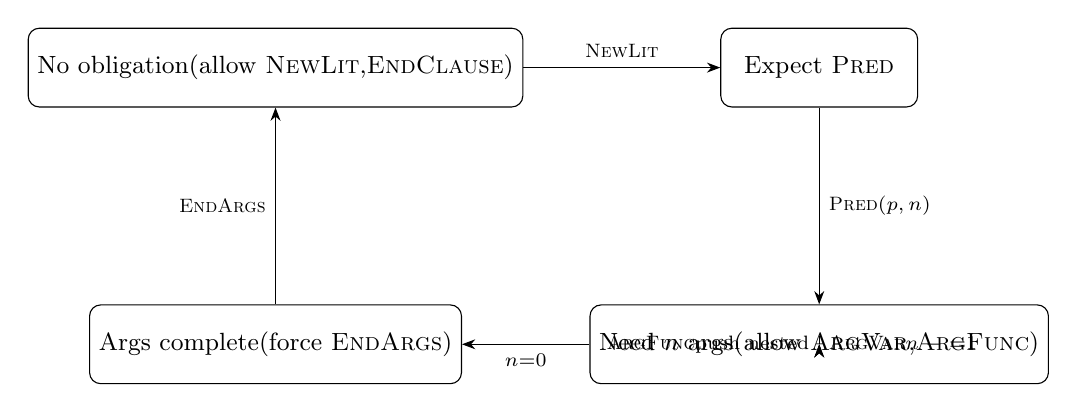
\begin{tikzpicture}[
    state/.style={rectangle, draw, rounded corners, minimum height=1cm,
                  minimum width=2.5cm, font=\small},
    >=Stealth,
    node distance=2.5cm
]
\node[state] (init) {No obligation\\(allow \textsc{NewLit},\\\textsc{EndClause})};
\node[state, right=of init] (pred) {Expect \textsc{Pred}};
\node[state, below=of pred] (args) {Need $n$ args\\(allow \textsc{ArgVar},\\\textsc{ArgFunc})};
\node[state, below=of init] (done) {Args complete\\(force \textsc{EndArgs})};

\draw[->] (init) -- node[above, font=\scriptsize] {\textsc{NewLit}} (pred);
\draw[->] (pred) -- node[right, font=\scriptsize] {\textsc{Pred}$(p, n)$} (args);
\draw[->] (args) -- node[below, font=\scriptsize] {$n{=}0$} (done);
\draw[->, bend left=20] (args) to node[right, font=\scriptsize] {\textsc{ArgVar}\\$n \mathrel{-}{=} 1$} (args);
\draw[->, bend right=40] (args) to node[left, font=\scriptsize] {\textsc{ArgFunc}\\push nested} (args);
\draw[->] (done) -- node[left, font=\scriptsize] {\textsc{EndArgs}} (init);

\end{tikzpicture}
\caption{State machine for arity-constrained decoding. Transitions show which
actions are allowed in each state. The stack handles nested function applications.}
\label{fig:arity_state}
\end{figure}

\end{document}
